Hoy en día no es prudente empezar un proyecto web sin una estrategia de respaldo. Debido a que los datos son efímeros y se pueden perder fácilmente, por ejemplo, a través de un cambio de código erróneo o un fallo catastrófico de disco, es aconsejable mantener un archivo de todo el trabajo.\\[0.8cm]
Para proyectos de texto y código, la estrategia de respaldo generalmente incluye control de versiones, o seguimiento y administración de revisiones.  Dado su papel fundamental, el control de versiones es más efectivo cuando se adapta a los hábitos y objetivos de trabajo del equipo del proyecto.\\[0.8cm]
En su forma más simple, un sistema de control de versiones proporciona un principio básico y un método para almacenar archivos y cambios realizados en ellos. Esto se logra mediante el uso de un repositorio. El repositorio contiene la versión más reciente de cada archivo y el historial de cambios que ha llevado a esa representación. Por lo general, cada cambio incluye información adicional, como el autor y una breve descripción.
\subsection{Git}
Git es un software de control de versiones distribuido particularmente potente, flexible y de bajo costo que hace que el desarrollo colaborativo sea un placer. \\[0.8cm]
La principal diferencia entre Git y cualquier otro versionador es la forma en que Git piensa acerca de sus datos. Conceptualmente, la mayoría de los otros sistemas almacenan información como una lista de cambios basados en archivos. Estos sistemas (CVS, Subversion, Perforce, Bazaar, etc.) piensan en la información que mantienen como un conjunto de archivos y los cambios realizados en cada archivo a lo largo del tiempo. Git no piensa ni almacena sus datos de esta manera. En cambio, Git piensa en sus datos más como un conjunto de instantáneas de un mini sistema de archivos. Cada vez que confirma o guarda el estado de su proyecto en Git, básicamente toma una fotografía de cómo se ven todos sus archivos en ese momento y almacena una referencia a esa instantánea. Para ser eficiente, si los archivos no han cambiado, Git no almacena el archivo nuevamente, solo un enlace al archivo idéntico anterior que ya ha almacenado. \\[0.8cm]
\begin{figure}[H]
  \centering
  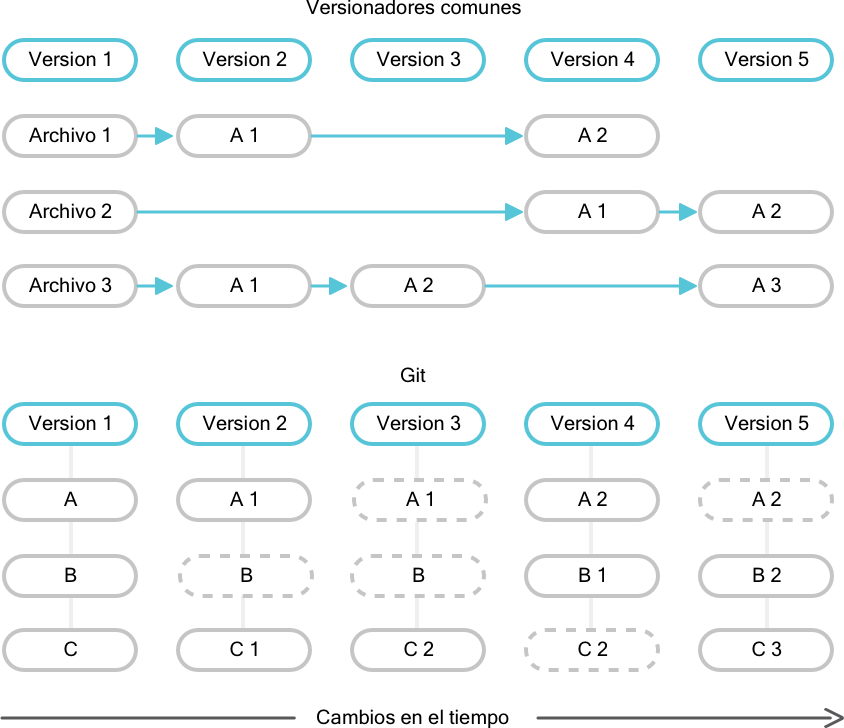
\includegraphics[width=0.9\textwidth]{git}
  \caption{Diferencias entre controladores de versiones. (Fuente: Elaboración propia)}
\end{figure}